\chapter{Case Study on Resource-centric Organizational Modeling}
\label{chap:casestudy}
In this chapter, we provide architecture of the functioning system as a first section. This section provides, implementation details along with the reason for making certain decisions regarding the implementation. The final section validates the system by  validating it with the proposed approach. This section also has some requirement evaluation with the state of the art.

%%%%%%%%%%%%%%%%%%%%%%%%%%%%%%%%%%%%%%%%%%%%%%%%%%%%%%%%%%%%%%%%%%%%%%%%%
\section{Presentation of the Functioning System}
\label{sec:presentationofthefunctioningsystem}
%%%%%%%%%%%%%%%%%%%%%%%%%%%%%%%%%%%%%%%%%%%%%%%%%%%%%%%%%%%%%%%%%%%%%%%%%

User interface URL navigation of the functioning system is provided in the Figure \ref{fig:UIArchitecture}


\begin{figure}
	\centering
	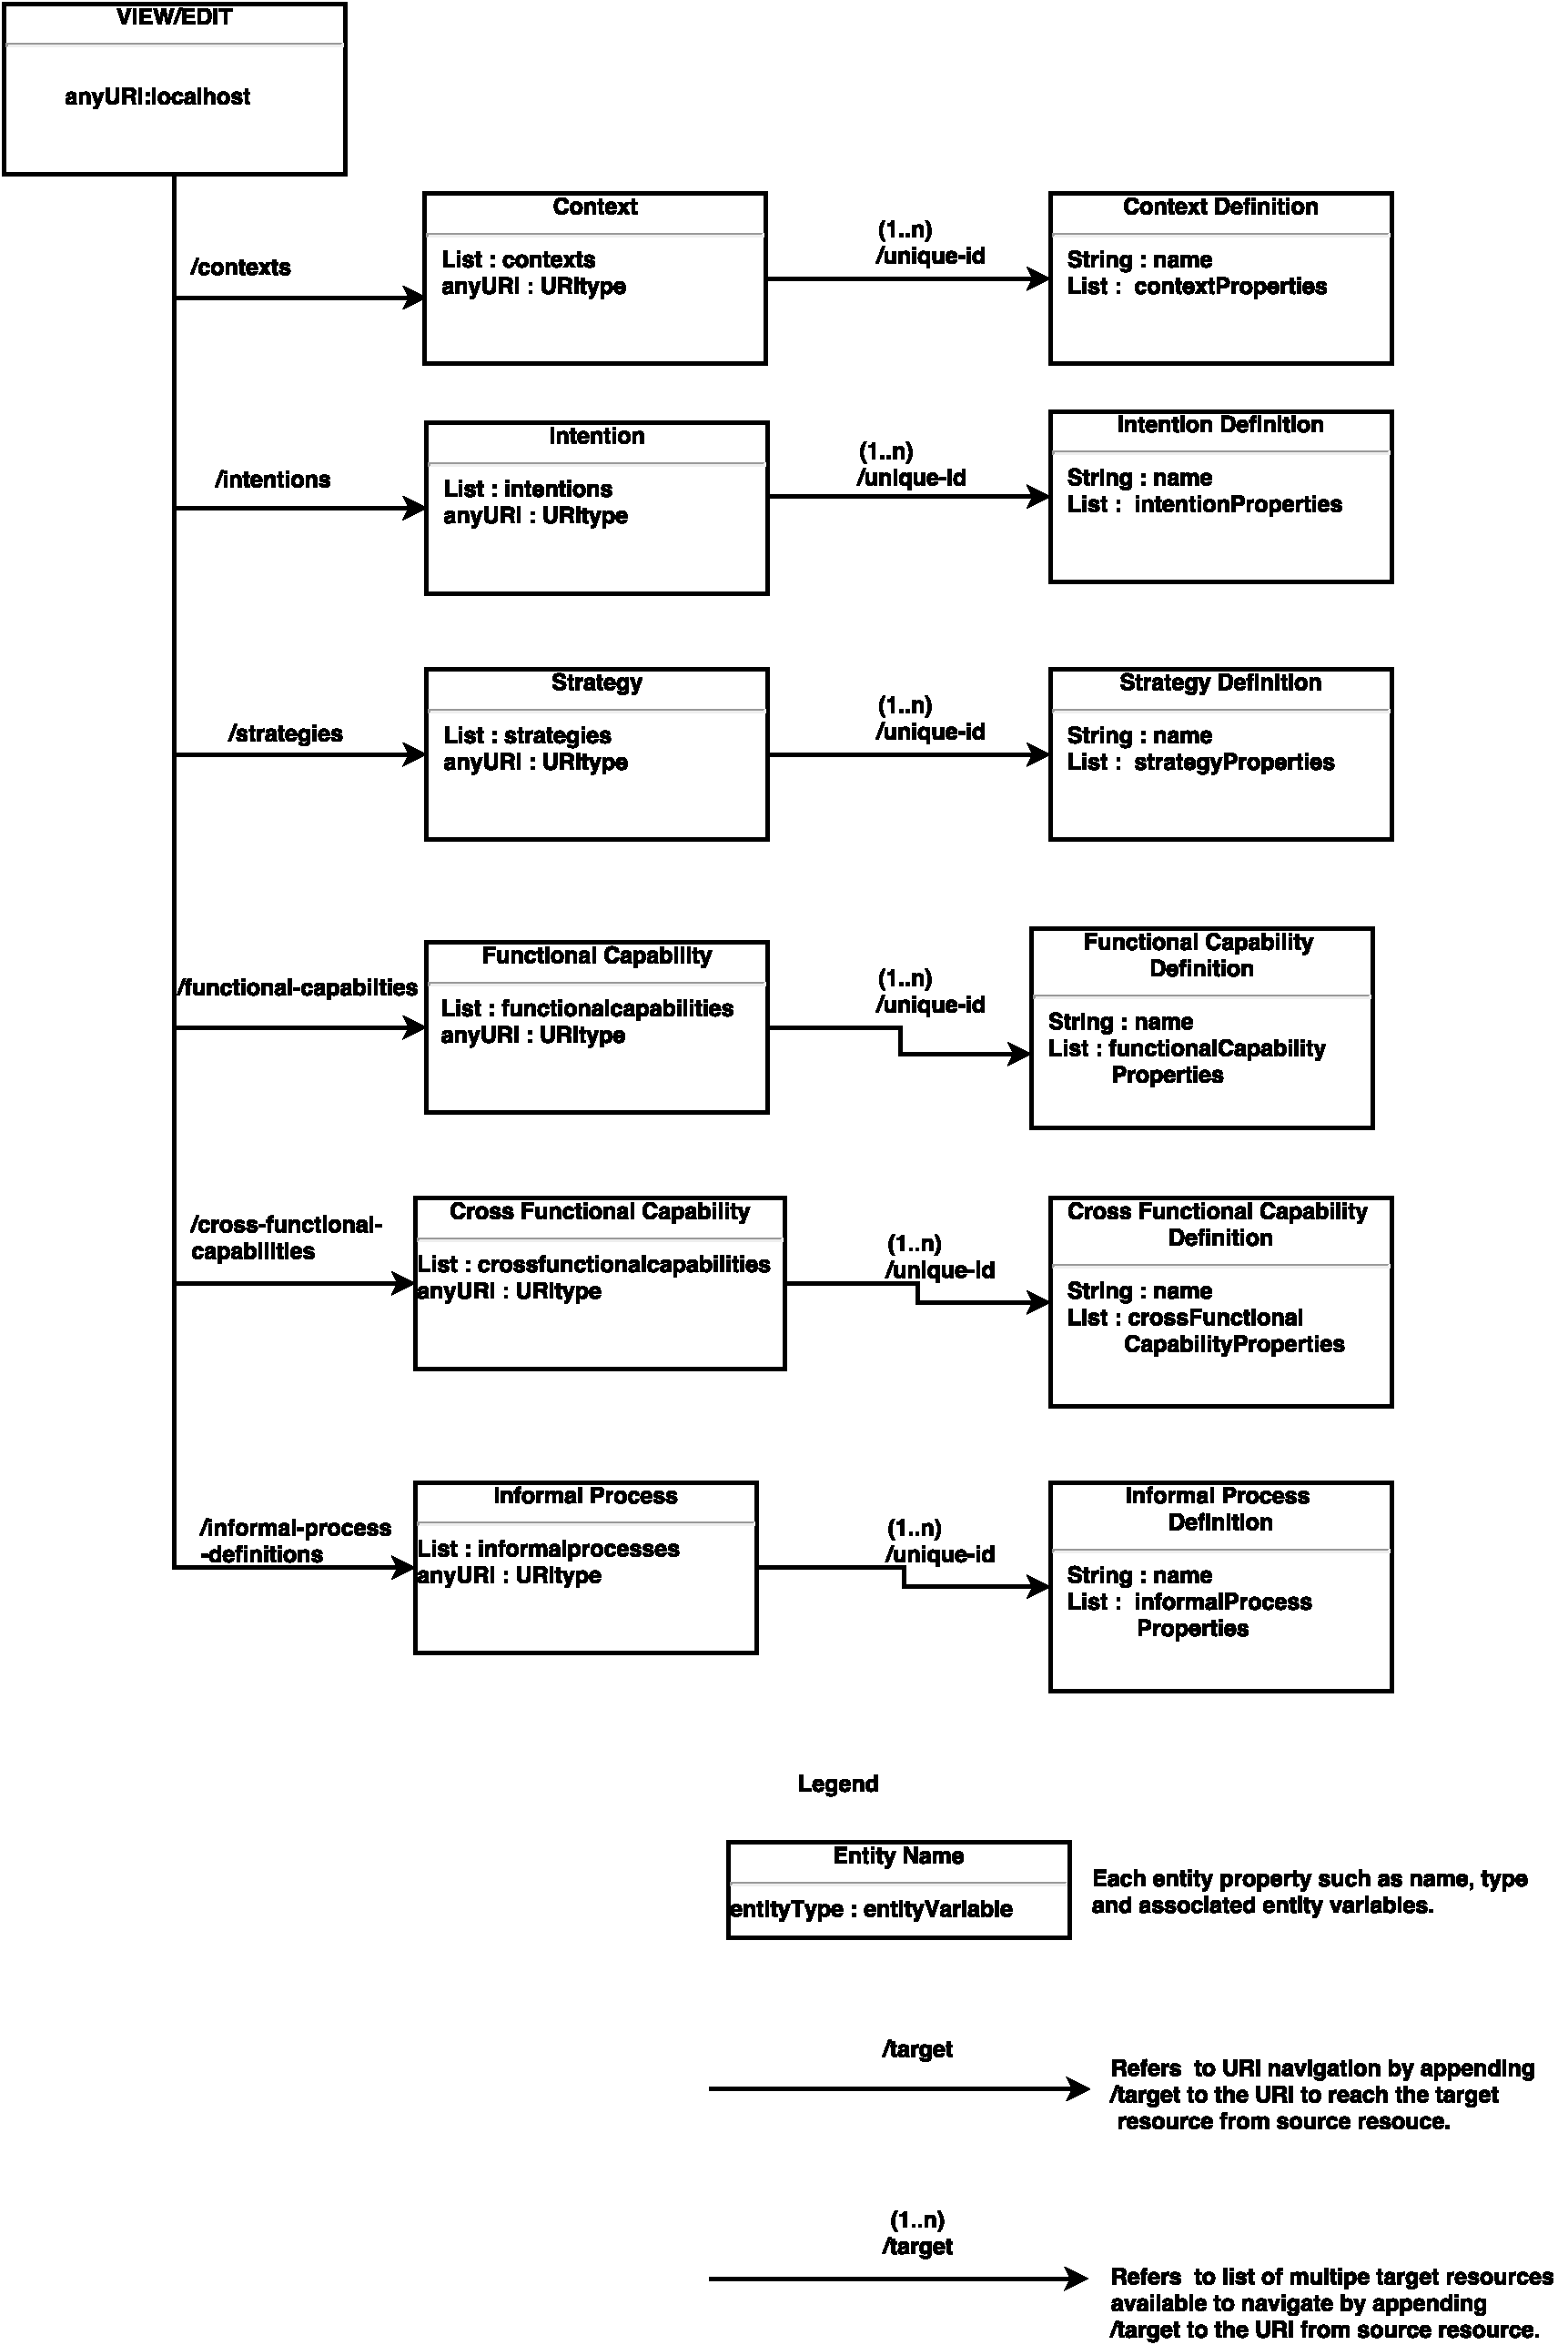
\includegraphics [width= \textwidth]{UIArchitecture.pdf}
	\caption{User interface URL navigation of the functioning system}
	\label{fig:UIArchitecture}
\end{figure}



%%%%%%%%%%%%%%%%%%%%%%%%%%%%%%%%%%%%%%%%%%%%%%%%%%%%%%%%%%%%%%%%%%%%%%%%%
\section{A Concrete View of Entity Types}
\label{sec:realization}
%%%%%%%%%%%%%%%%%%%%%%%%%%%%%%%%%%%%%%%%%%%%%%%%%%%%%%%%%%%%%%%%%%%%%%%%%
%how did I implement, technology and frameworks used and why.
It is important to discuss the conrete concepts of informal process from an organizational aspect, because they have a direct effect on the outcome of the informal process \cite{Sungur2014}. This section discusses about how Intention-centric organizational modeling realized as an user interface editor  from an organizational aspect by taking the motivating scenario discussed in Chapter \ref {chap:motivatingScenario}. 



%%%%%%%%%%%%%%%%%%%%%%%%%%%%%%%%%%%%%%%%%%%%%%%%%%%%%%%%%%%%%%%%%%%%%%%%%
\subsection{Realization of Entity Views}
\label{subsec:realofentityviews}
%%%%%%%%%%%%%%%%%%%%%%%%%%%%%%%%%%%%%%%%%%%%%%%%%%%%%%%%%%%%%%%%%%%%%%%%%
The XML Schema Definition of entity type has been provided in \ref{lst:xsdlist}



\begin{Listing}
	\begin{lstlisting}
	<xs:complexType name="tEntityType" abstract="true">
	<xs:complexContent>
	<xs:extension base="tExtensibleElements">
	<xs:sequence>
	<xs:element name="Tags" type="tTags" minOccurs="0"/>
	<xs:element name="DerivedFrom" minOccurs="0">
	<xs:complexType>
	<xs:attribute name="typeRef" type="xs:QName" use="required"/>
	</xs:complexType>
	</xs:element>
	<xs:element name="PropertiesDefinition" minOccurs="0">
	<xs:complexType>
	<xs:attribute name="element" type="xs:QName"/>
	<xs:attribute name="type" type="xs:QName"/>
	</xs:complexType>
	</xs:element>
	</xs:sequence>
	<xs:attribute name="name" type="xs:NCName" use="required"/>
	<xs:attribute name="abstract" type="tBoolean" default="no"/>
	<xs:attribute name="final" type="tBoolean" default="no"/>
	<xs:attribute name="targetNamespace" type="xs:anyURI" use="optional"/>
	</xs:extension>
	</xs:complexContent>
	</xs:complexType>>
	\end{lstlisting}
	\caption{XML Schema Definition of Entity Type}
	\label{lst:xsdlist}
\end{Listing}

%%%%%%%%%%%%%%%%%%%%%%%%%%%%%%%%%%%%%%%%%%%%%%%%%%%%%%%%%%%%%%%%%%%%%%%%%
\subsection{Realization of Organizational Intentions}
%%%%%%%%%%%%%%%%%%%%%%%%%%%%%%%%%%%%%%%%%%%%%%%%%%%%%%%%%%%%%%%%%%%%%%%%%


%%%%%%%%%%%%%%%%%%%%%%%%%%%%%%%%%%%%%%%%%%%%%%%%%%%%%%%%%%%%%%%%%%%%%%%%%
\subsection{Realization of Organizational  Strategies}
%%%%%%%%%%%%%%%%%%%%%%%%%%%%%%%%%%%%%%%%%%%%%%%%%%%%%%%%%%%%%%%%%%%%%%%%%

%%%%%%%%%%%%%%%%%%%%%%%%%%%%%%%%%%%%%%%%%%%%%%%%%%%%%%%%%%%%%%%%%%%%%%%%%
\subsection{Realization of Organizational Capabilities}
%%%%%%%%%%%%%%%%%%%%%%%%%%%%%%%%%%%%%%%%%%%%%%%%%%%%%%%%%%%%%%%%%%%%%%%%%
There are two types of capabilities. Functional capabilities and cross-functional capabilities. Functional capabilities must be associated with instance descriptors. Cross-functional capabilities are capabilities containing multiple functional capabilities. We need to have the ability to add and remove instance descriptors for an entity type, e.g, resource definitions,  informal process definitions, etc. An instance descriptor of a functional capability should refer to a resource definition meaning that a capability is provided by a resource definition. So an instance descriptor of a capability refers to a resource definition and we can manually add and remove resource definitions in general.




%%%%%%%%%%%%%%%%%%%%%%%%%%%%%%%%%%%%%%%%%%%%%%%%%%%%%%%%%%%%%%%%%%%%%%%%%
\subsection{Realization of Organizational Resources}
%%%%%%%%%%%%%%%%%%%%%%%%%%%%%%%%%%%%%%%%%%%%%%%%%%%%%%%%%%%%%%%%%%%%%%%%%
There are two keys, one for tosca repository and one for tosca modeling tool. Tosca repository url refers to winery and the other one refers to topology modeler. This should only contain root contexts and additional suffixes such as service templates in a separate key in default db.Out of these a function should create corresponding url for topology modeling. The topology modeler page of a specific service temple without knowing its id and namespace. This can be composed from different variables: :topology-modeler-url, :tosco-repository-url,:target-namespace, and :id.


\fbox{
	\begin{minipage}{\textwidth}
		\{topology-modeler-url\}?repositoryURL=\{encoded-tosca-repository-url\}\&ns=\{encoded-target-namepsace\}\&id=\{encoded-id\}\#
	\end{minipage}
	}
	
		
What important is, at the end editor should have a view that is capable of adding, viewing, deleting and updating models aligned with the XSD schema. In general, separate entities should reference each other but not contain each other. For instance, a strategy containing a goal should use goals id to resolve it but not the actual goal.
	
%%%%%%%%%%%%%%%%%%%%%%%%%%%%%%%%%%%%%%%%%%%%%%%%%%%%%%%%%%%%%%%%%%%%%%%%%
	\subsection{Realization of Informal Processes}
%%%%%%%%%%%%%%%%%%%%%%%%%%%%%%%%%%%%%%%%%%%%%%%%%%%%%%%%%%%%%%%%%%%%%%%%%
	
	
	
%%%%%%%%%%%%%%%%%%%%%%%%%%%%%%%%%%%%%%%%%%%%%%%%%%%%%%%%%%%%%%%%%%%%%%%%%
\section{Validation}
\label{sec:validation}
%%%%%%%%%%%%%%%%%%%%%%%%%%%%%%%%%%%%%%%%%%%%%%%%%%%%%%%%%%%%%%%%%%%%%%%%%	
This section validates the degree of satisfaction of the research objectives discussed in Chapter \ref{chap:introduction} against the developed prototype through. Also, we claim that this master thesis is a part of creating models that are required for supporting and automating informal processes, it is important to evaluate the developed prototype along with the requirements that are discussed in the approach \textit{Informal Process Essentials} \cite{Sungur2014a}. In this section, examples are provided from motivating scenario which is discussed in the Chapter \ref{chap:motivatingScenario}.
		
%%%%%%%%%%%%%%%%%%%%%%%%%%%%%%%%%%%%%%%%%%%%%%%%%%%%%%%%%%%%%%%%%%%%%%%%%
\subsection{Validation of Research Objectives}
\label{subsec:validationofrequirements}
%%%%%%%%%%%%%%%%%%%%%%%%%%%%%%%%%%%%%%%%%%%%%%%%%%%%%%%%%%%%%%%%%%%%%%%%%
As discussed in Chapter \ref{chap:approach}, the research objectives are satisfied at the design level but their validity can be confirmed only by evaluating the research objectives with some sample scenarios provided in Chapter \ref{chap:motivatingScenario}.   

\textit{Organizational intentions transparency} (R1): A valid user whose credentials are stored in database is able to login successfully and view the intentions and its associated entities. Hence the research objective R1 is met.

\textit{Organizational intention resource-based cost estimation} (R2): An intention whose cost is unspecified for a sample intention, is calculated by the developed system recursively as mentioned in the Chapter \ref{chap:approach}. Thus the research objective R2 is also met.

\textit{Organizational intention achievability estimation} (R3): Similar to cost calculation, an intention instance whose achievability is not in prior is also estimated by the current functioning system. Hence research objective R3 is satisifed.

\textit{Intention oriented working style} (R4): The users can login and create intention models, strategy models, informal process models etc., through the developed editor. Hence research objective R4 is also met.

\textit{Participative organizational modeling} (R5): Each entity type that can be interactively acquirable has list of participants with their corresponding privileges. Thus this satisfies the requirements of research objective R5.

\textit{Re-use of organizational knowledge} (R6): The descriptive information about each models can be stored and re-used for next enactments. Hence research objective R6 is also met.
	
%%%%%%%%%%%%%%%%%%%%%%%%%%%%%%%%%%%%%%%%%%%%%%%%%%%%%%%%%%%%%%%%%%%%%%%%%
\subsection{Validation of Prototype}
\label{subsec:validationofprototype}
%%%%%%%%%%%%%%%%%%%%%%%%%%%%%%%%%%%%%%%%%%%%%%%%%%%%%%%%%%%%%%%%%%%%%%%%%
In the approach of \textit{Supporting Informal Processes} \cite{Sungur2014}, the author has categorized generic requirements that supports enactment of informal processes under three dimensions such as business logic, IT infrastructure and organization. In order to make the validation procedure simple, we have taken the concrete requirements discussed in the approach of \textit{Informal Process Essentials} \cite{Sungur2014a}. This is because the latter approach itself is an extended work of former approach.  

\textit{Enactable Informal Process Representation}: In this requirement, the core elements are performers, IT tools, data etc., and the requirement gets satisfied only when we are able to provide textual descriptions of how to make these ready. In the functioning web editor, the user can create textual information i.e models required for resources, contexts, strategies etc. Hence the developed prototype satisfies the requirement of providing enactable informal process representation. For example, using our motivating scenario we only provide definitions of intentions, contexts, strategies, capabilities and resources inside the editor but there is no functionality to  predefine business logic of these informal processes.

\textit{Resource Relationships Definition}: In an informal process, each resource can have a relation with other resource. For example in our motivating scenario, a resource with front-end developer capability has a "requires" relationship with front-end developer tools. In the functioning system, Winery modeling tool's repository web page has been included to edit the resource models. Thus the functioning system also satisfies the requirement of defining relationship between the resources. 

\textit{Resource Visibility Definition}: Informal processes contains resources that work towards the process' specific intention. These resources can participate in more than one informal process. For example, in the same organization as in our motivating scenario there can be another process working towards achieving an intention say \textit{improving skills of all the employees}. This can make an employee with a developer capability to participate in both the processes. Thus all the resources of an informal process has to be visible. In or functioning system we have septate user interface tab that details associated resources of an informal process. This satisfies the requirement of making the resource definitions visible.    

\textit{Support for Dynamically Changing Resources}: Due to dynamic nature of informal processes, the developed editor provides facility to add or remove resources. For example, in our motivating scenario consider the sub-intention of \textit{improving the help desk portal} where a new requirement of \textit{extending the help desk portal support in mobiles} may arise dynamically. In this situation, the editor must provide means to add new resource with new capability of \textit{mobile application developer capability}. The functioning system provides facility to add or remove resources associated with capabilities. Thus the requirement of providing support for dynamically changing resources is also satisfied by the editor. 
	


